\begin{question}
\noindent A school's Design Technology club is building a rectangular laboratory frame, $ABCDEFGH$, for a UI/UX display stand. The base $ABCD$ is a rectangle with $AB = 9$ cm and $BC = 5$ cm. The frame has a vertical height $CG = 7$ cm, as shown in the diagram.

\begin{center}
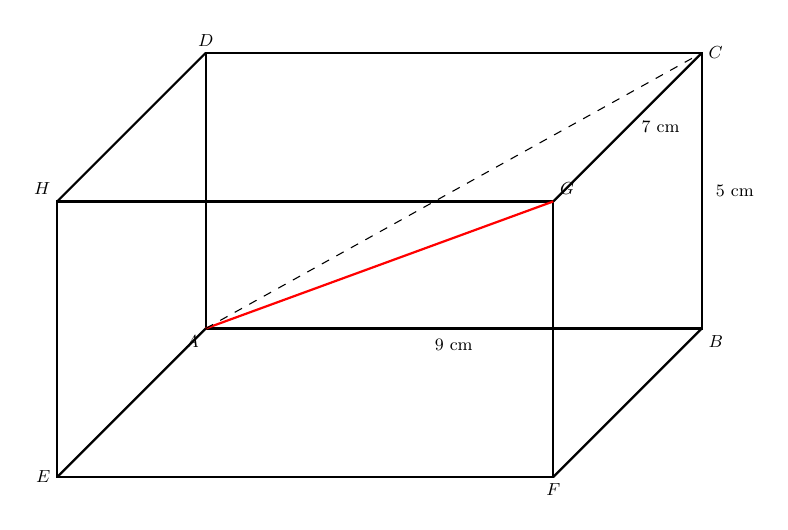
\begin{tikzpicture}[scale=0.7, transform shape]
    % Base rectangle ABCD
    \coordinate (A) at (0,0,0);
    \coordinate (B) at (9,0,0);
    \coordinate (C) at (9,5,0);
    \coordinate (D) at (0,5,0);
    % Top rectangle EFGH (directly above)
    \coordinate (E) at (0,0,7);
    \coordinate (F) at (9,0,7);
    \coordinate (G) at (9,5,7);
    \coordinate (H) at (0,5,7);

    % Draw base
    \draw[thick] (A) -- (B) -- (C) -- (D) -- cycle;
    % Draw top
    \draw[thick] (E) -- (F) -- (G) -- (H) -- cycle;
    % Vertical edges
    \draw[thick] (A) -- (E);
    \draw[thick] (B) -- (F);
    \draw[thick] (C) -- (G);
    \draw[thick] (D) -- (H);

    % Diagonal support rod from A to G
    \draw[thick, red] (A) -- (G);
    % Diagonal of base from A to C (dashed, for construction)
    \draw[dashed] (A) -- (C);

    % Labels
    \node at (A) [below left, font=\small] {$A$};
    \node at (B) [below right, font=\small] {$B$};
    \node at (C) [right, font=\small] {$C$};
    \node at (D) [above, font=\small] {$D$};
    \node at (E) [left, font=\small] {$E$};
    \node at (F) [below, font=\small] {$F$};
    \node at (G) [above right, font=\small] {$G$};
    \node at (H) [above left, font=\small] {$H$};

    \node at (4.5,-0.3,0) [font=\small] {$9$ cm};
    \node at (9.6,2.5,0) [font=\small] {$5$ cm};
    \node at (9.6,5,3.5) [font=\small] {$7$ cm};
\end{tikzpicture}
\end{center}

\noindent A diagonal support rod is fixed from corner $A$ (on the base) to corner $G$ (diagonally opposite, at the top of the frame), as shown in red.

\noindent Find the angle that the rod $AG$ makes with the base $ABCD$, giving your answer correct to 1 decimal place.

\vspace{6cm}

\begin{flushright}
    \answerequnit{x}{$^\circ$}{4}
\end{flushright}
\end{question}
